\documentclass[tikz,border=8pt]{standalone}
% Shared look for every TikZ diagram. Load with % Shared look for every TikZ diagram. Load with % Shared look for every TikZ diagram. Load with \input{../../tools/tikz-style.tex}
\usepackage[T1]{fontenc}
\usepackage{lmodern}
\renewcommand{\sfdefault}{lmr}  % diagrams use the same serif as the text
\usetikzlibrary{arrows.meta, positioning, shapes.geometric, calc, fit, backgrounds}
\definecolor{cblue}{HTML}{4C78A8}
\definecolor{corange}{HTML}{F58518}
\definecolor{cgreen}{HTML}{54A24B}
\definecolor{cred}{HTML}{E45756}
\definecolor{cpurple}{HTML}{B279A2}
\definecolor{cgrey}{HTML}{6B6B6B}
\tikzset{
  every picture/.style={font=\sffamily, line width=1.2pt},
  box/.style={draw=#1, fill=#1!12, rounded corners=4pt, align=center, inner sep=7pt, minimum height=1.1cm},
  box/.default=cgrey,
  arrow/.style={-{Stealth[length=3mm]}, draw=cgrey, line width=1.4pt},
  title/.style={font=\sffamily\bfseries\Large},
  note/.style={font=\sffamily\small, text=cgrey, align=center},
}
\AtBeginDocument{\hyphenpenalty=10000 \exhyphenpenalty=10000}

\usepackage[T1]{fontenc}
\usepackage{lmodern}
\renewcommand{\sfdefault}{lmr}  % diagrams use the same serif as the text
\usetikzlibrary{arrows.meta, positioning, shapes.geometric, calc, fit, backgrounds}
\definecolor{cblue}{HTML}{4C78A8}
\definecolor{corange}{HTML}{F58518}
\definecolor{cgreen}{HTML}{54A24B}
\definecolor{cred}{HTML}{E45756}
\definecolor{cpurple}{HTML}{B279A2}
\definecolor{cgrey}{HTML}{6B6B6B}
\tikzset{
  every picture/.style={font=\sffamily, line width=1.2pt},
  box/.style={draw=#1, fill=#1!12, rounded corners=4pt, align=center, inner sep=7pt, minimum height=1.1cm},
  box/.default=cgrey,
  arrow/.style={-{Stealth[length=3mm]}, draw=cgrey, line width=1.4pt},
  title/.style={font=\sffamily\bfseries\Large},
  note/.style={font=\sffamily\small, text=cgrey, align=center},
}
\AtBeginDocument{\hyphenpenalty=10000 \exhyphenpenalty=10000}

\usepackage[T1]{fontenc}
\usepackage{lmodern}
\renewcommand{\sfdefault}{lmr}  % diagrams use the same serif as the text
\usetikzlibrary{arrows.meta, positioning, shapes.geometric, calc, fit, backgrounds}
\definecolor{cblue}{HTML}{4C78A8}
\definecolor{corange}{HTML}{F58518}
\definecolor{cgreen}{HTML}{54A24B}
\definecolor{cred}{HTML}{E45756}
\definecolor{cpurple}{HTML}{B279A2}
\definecolor{cgrey}{HTML}{6B6B6B}
\tikzset{
  every picture/.style={font=\sffamily, line width=1.2pt},
  box/.style={draw=#1, fill=#1!12, rounded corners=4pt, align=center, inner sep=7pt, minimum height=1.1cm},
  box/.default=cgrey,
  arrow/.style={-{Stealth[length=3mm]}, draw=cgrey, line width=1.4pt},
  title/.style={font=\sffamily\bfseries\Large},
  note/.style={font=\sffamily\small, text=cgrey, align=center},
}
\AtBeginDocument{\hyphenpenalty=10000 \exhyphenpenalty=10000}

\begin{document}
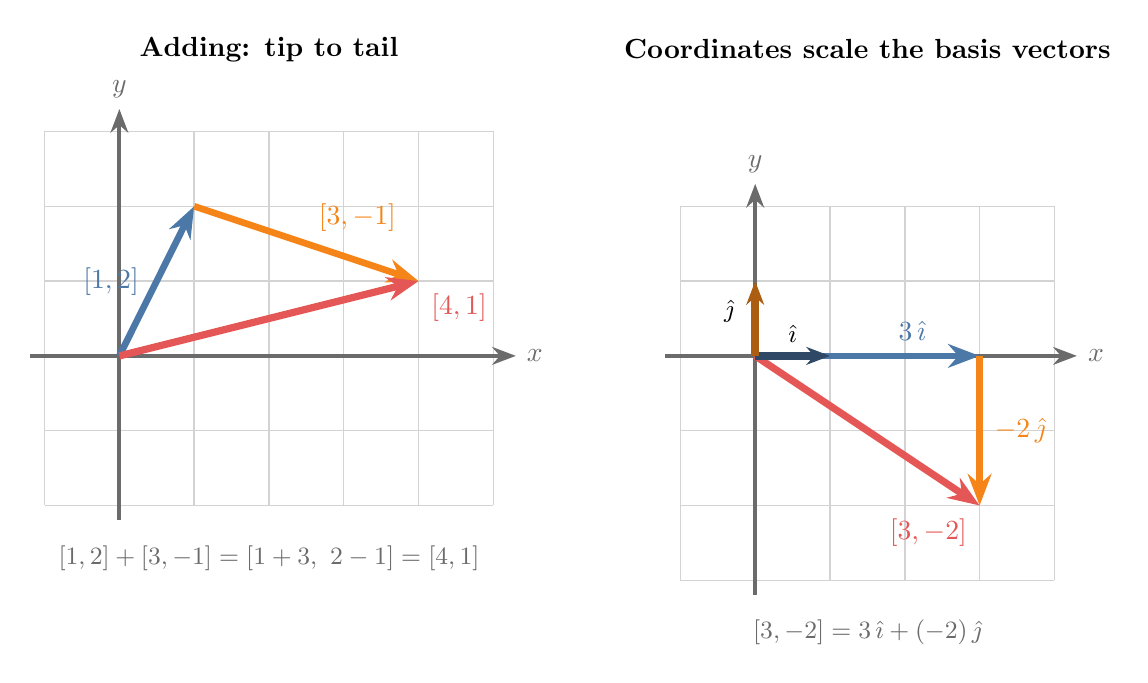
\begin{tikzpicture}[scale=0.95]
  \begin{scope}
    \node[font=\bfseries] at (2,4.1) {Adding: tip to tail};
    \draw[cgrey!30, line width=0.5pt] (-1,-2) grid (5,3);
    \draw[arrow, cgrey] (-1.2,0) -- (5.3,0) node[right] {$x$};
    \draw[arrow, cgrey] (0,-2.2) -- (0,3.3) node[above] {$y$};
    \draw[-{Stealth[length=4mm]}, cblue, line width=2.4pt] (0,0) -- (1,2) node[midway, left=2pt, font=\bfseries] {$[1, 2]$};
    \draw[-{Stealth[length=4mm]}, corange, line width=2.4pt] (1,2) -- (4,1) node[midway, above right=0pt, font=\bfseries] {$[3, -1]$};
    \draw[-{Stealth[length=4mm]}, cred, line width=2.6pt] (0,0) -- (4,1) node[below right=0pt, font=\bfseries] {$[4, 1]$};
    \node[note] at (2,-2.7) {$[1, 2] + [3, -1] = [1 + 3,\ 2 - 1] = [4, 1]$};
  \end{scope}
  \begin{scope}[xshift=8.5cm]
    \node[font=\bfseries] at (1.5,4.1) {Coordinates scale the basis vectors};
    \draw[cgrey!30, line width=0.5pt] (-1,-3) grid (4,2);
    \draw[arrow, cgrey] (-1.2,0) -- (4.3,0) node[right] {$x$};
    \draw[arrow, cgrey] (0,-3.2) -- (0,2.3) node[above] {$y$};
    \draw[-{Stealth[length=4mm]}, cblue, line width=2.4pt] (0,0) -- (3,0) node[pos=0.7, above=1pt, font=\bfseries] {$3\,\hat{\imath}$};
    \draw[-{Stealth[length=4mm]}, corange, line width=2.4pt] (3,0) -- (3,-2) node[midway, right=1pt, font=\bfseries] {$-2\,\hat{\jmath}$};
    \draw[-{Stealth[length=4mm]}, cred, line width=2.6pt] (0,0) -- (3,-2) node[below left=0pt, font=\bfseries] {$[3, -2]$};
    \draw[-{Stealth[length=3mm]}, cblue!60!black, line width=3pt] (0,0) -- (1,0);
    \draw[-{Stealth[length=3mm]}, corange!70!black, line width=3pt] (0,0) -- (0,1);
    \node[font=\small, fill=white, inner sep=1pt] at (-0.35,0.6) {$\hat{\jmath}$};
    \node[font=\small, fill=white, inner sep=1pt] at (0.5,0.3) {$\hat{\imath}$};
    \node[note] at (1.5,-3.7) {$[3, -2] = 3\,\hat{\imath} + (-2)\,\hat{\jmath}$};
  \end{scope}
\end{tikzpicture}
\end{document}
